\documentclass{beamer}
\usepackage[utf8]{inputenc}
\usepackage[T1]{fontenc}
\usepackage[francais]{babel} 
\usepackage{lmodern}
\usepackage{hyperref}
\usepackage{tikz}
\usepackage{tabularx, longtable}

\usetikzlibrary{trees,shapes.geometric,arrows,decorations.pathmorphing,backgrounds,fit,positioning,shapes.symbols,chains	}
 \tikzset{
    %Define standard arrow tip
    >=stealth',
    %Define style for boxes
    punkt/.style={
           rectangle, dashed,
           rounded corners,
           draw=black, very thin,
           minimum height=2em,
           minimum width = 2cm,
           text centered},
    square/.style={
           rectangle,
           draw=black, thick,
           minimum height=.5cm,
           text centered},
    data/.style={
           rectangle,
           draw=black, thick,
           minimum height= 2cm,
           minimum width = 2cm,
           text centered},
    % Define arrow style
    pil/.style={
           ->,
           thick,
           shorten <=1pt,
           shorten >=1pt,},
    asym/.style={
           <->,
           thin,
           shorten <=1pt,
           shorten >=1pt,
           red!100},
    sym/.style={
           <->,
           thin,
           shorten <=1pt,
           shorten >=1pt,
           blue!100}
}
\usepackage{pgfplots}
\usepackage{eurosym}
\usepackage{rotating}
\usepackage{array}


\usetikzlibrary{shapes,arrows}
\usetikzlibrary{positioning}
\usetikzlibrary{calc, shadings, shadows, shapes.arrows,shapes.multipart,decorations.pathreplacing,shapes.symbols}
\usetikzlibrary{trees,shapes.geometric,arrows,decorations.pathmorphing,backgrounds,fit,positioning,shapes.symbols,chains        }
\tikzset{%
  interface/.style={draw, rectangle, rounded corners, font=\LARGE\sffamily},
  ethernet/.style={interface, fill=yellow!50, font=\tiny},% ethernet interface
  serial/.style={interface, fill=green!70},% serial interface
  network/.style={sloped, anchor=south, font=\footnotesize\sffamily, color=black!50!green,outer sep=.2cm},% line speed at edge
  network2/.style={anchor=east, font=\tiny\sffamily, color=black!50!green},% line speed at edge
  networkname/.style={sloped, anchor=north, font=\tiny\sffamily, color=black!50!green},% line speed at edge
  networkname2/.style={anchor=west, font=\tiny\sffamily, color=black!50!green},% line speed at edge
  route/.style={draw, shape=single arrow, single arrow head extend=4mm,
    minimum height=1.7cm, minimum width=3mm, white, fill=gray!20,
    drop shadow={opacity=.8, fill=gray!50!black}, font=\tiny},% inroute / outroute arrows
  address/.style={color=red, font=\small\sffamily}
}

\usetheme{Antibes}
\usecolortheme{beaver}
\setbeamertemplate{sections/subsections in toc}[square]
\setbeamertemplate{blocks}[square]%

\author{Julien Bourdon - Julien Legras - Jean-Baptiste Souchal}
\title{Administration réseaux - Les systèmes de détection d'intrusion}
\titlegraphic{\includegraphics[height=3em]{logo_univ.png}}
\institute{Master 2 Sécurité des Systèmes Informatiques}

\date{17/01/2014}

\begin{document}

{
\setbeamertemplate{headline}[default] 
\begin{frame}
  \titlepage
\end{frame}
}

%% JB
\frame{
\frametitle{Sommaire}
\tableofcontents
}

\section{Présentation générale}
\subsection{Les IDS}
\frame[allowframebreaks=1.0]{
\frametitle{Les IDS}
\begin{block}{Objectifs des IDS}
\begin{itemize}
\item Surveiller
\item Contrôler
\item Détecter
\item Sniffer \& analyser
\end{itemize}
\end{block}

\begin{block}{Domaines d'analyse}
\begin{itemize}
\item Couche réseau (IP, ICMP)
\item Couche transport (TCP, UDP)
\item Couche application (HTTP, telnet)
\end{itemize}
\end{block}

\framebreak

\begin{block}{Types}
\begin{itemize}
\item HIDS
\item NIDS
\end{itemize}
\end{block}

\begin{block}{Actions}
\begin{itemize}
\item Journaliser
\item Avertir (système, humain)
\item Agir (fin de connexion...)
\end{itemize}
\end{block}


\framebreak

\begin{block}{Méhodes de détection}
\begin{itemize}
\item Signature
    \begin{itemize}
        \item Expressions régulières
        \item Comparaison avec les signatures connues
    \end{itemize}
\item Comportementale
    \begin{itemize}
        \item Détection d'anomalie
        \item Vérification d'intégrité
    \end{itemize}
\end{itemize}
\end{block}

\begin{alertblock}{Dangers}
\begin{itemize}
\item Faux-positifs
\item Faux-négatifs
\item[] $\hookrightarrow$ Evasion
\end{itemize}
\end{alertblock}

}

\subsection{Les IPS}
\frame{
\frametitle{Les IPS}
\begin{block}{Fonctionnalités}
\begin{itemize}
\item IDS avec fonction de blocage
\item Interrompre ou ralentir la connexion
\item Blacklister une source
\item Attention aux faux-positifs
\end{itemize}
\end{block}
}



%% JBOURDON
\section{Snort}
\frame{
\frametitle{Introduction}
\begin{center}
    \includegraphics[width=4cm]{icons/LogoSnort.jpg}
\end{center}
\begin{block}{Snort}
\begin{itemize}
\item IDS le plus utilisé ($\sim$ 2 millions de téléchargements)
\item Création en 1998 par Marty Roesh
\item Open source
\item Association possible avec un pare-feu
\end{itemize}
\end{block}

}

\subsection{Fonctionnalités}
\frame[allowframebreaks=1.0]{
\frametitle{Fonctionnalités}

\begin{block}{Architecture}
\begin{itemize}
\item Décodeur de paquets
\item Pré-processeurs
\item Moteur de détection
\item Système d'alerte et d'enregistrement
\item Modules de sortie
\end{itemize}
\end{block}

\framebreak
\begin{columns}[t]
    \begin{column}{.5\linewidth}
        \begin{block}{Actions en mode IDS}
            \begin{itemize}
                \item alert
                \item log
                \item pass
                \item activate
                \item dynamic
            \end{itemize}
        \end{block}
    \end{column}
    \begin{column}{.5\linewidth}
        \begin{block}{Actions en mode IPS}
            \begin{itemize}
                \item drop
                \item reject
                \item sdrop
            \end{itemize}
        \end{block}
    \end{column}
\end{columns}

\framebreak

\begin{block}{Éléments d'une règle}
\begin{itemize}
\item Une action
\item Un protocole
\item (Adresse source, port source) et (adresse destination, port destination)
\item Un opérateur indiquant la direction du flux (-> ou <>)
\end{itemize}
\end{block}


\begin{exampleblock}{Exemple}
\color{red}alert \color{black!30!green}tcp \color{blue} any \color{blue!60!red}any \color{orange}<> \color{blue}192.168.1.0/24 \color{blue!60!red}any \color{black}(content-list:"adults"; msg: "Adults list access attempt"; react: block;)

\color{red}action	\color{black}/ \color{black!30!green}protocole \color{black}/ \color{blue}adresse IP \color{black}/ \color{blue!60!red}port \color{black}/ \color{orange}opérateur
\end{exampleblock}

\framebreak

\begin{block}{Quelques champs utiles}
\begin{itemize}
\item msg
\item sid
\item classtype
\item priority
\item content
\item uricontent
\end{itemize}
\end{block}

\framebreak

\begin{exampleblock}{Exemple de type personnalisé}
\begin{verbatim}
ruletype redalert
{
    type alert 
    output alert_syslog: LOG_AUTH LOG_ALERT 
    output log_tcpdump: suspicious.log
}
\end{verbatim}
\end{exampleblock}

}


%% JLEGRAS
\section{Suricata}
\frame{
\frametitle{Introduction}
\begin{center}
    \includegraphics[width=3cm]{icons/suricata.png}
\end{center}
\begin{block}{Suricata}
\begin{itemize}
\item IDS jeune mais actif
\item Soutenu par The Open Information Security Foundation (OISF)
\item Open source
\end{itemize}
\end{block}

%\framebreak

%\begin{columns}[t]
%    \begin{column}{.5\linewidth}
%        \begin{block}{Suricata}
%            \begin{itemize}
%                \item soutenu par une fondation
%                \item multi-threadé
%                \item IPS natif
%                \item fonctions avancées (flowint, libHTP)
%                \item support de PF\_RING
%                \item code moderne et modulaire
%                \item jeune mais dynamique
%            \end{itemize}
%        \end{block}
%    \end{column}
%    \begin{column}{.5\linewidth}
%        \begin{block}{Snort}
%            \begin{itemize}
%                \item développé par Sourcefire
%                \item multi-processus
%                \item IPS supporté
%                \item jeu de règles SO (+ performances mais fermé)
%                \item pas d’accélération matérielle
%                \item code vieillissant
%                \item 10 ans d’expérience

%            \end{itemize}
%        \end{block}
%   \end{column}
%\end{columns}

}

\subsection{Fonctionnalités}
\frame[allowframebreaks=1.0]{
\frametitle{Fonctionnalités}

\begin{block}{Fonctionnalités modernes}
\begin{itemize}
\item Support natif de l’IPv6
\item Multi-threadé
\item Accélération matérielle native (GPU avec CUDA, PF\_RING)
\item IPS natif
\item Paramétrage CPU
\begin{itemize}
    \item Affectation d’un thread à un CPU
    \item Affectation d’une famille de threads à un ensemble de CPU
    \item Prise en compte des interruptions matérielles
\end{itemize}
\item Extraction et l’inspection de fichiers
\item Analyse de handshake TLS
\end{itemize}
\end{block}

\framebreak

\begin{columns}[t]
    \begin{column}{.5\linewidth}
        \begin{block}{Modules d'entrée IDS}
            \begin{itemize}
                \item PCAP
                    \begin{itemize}
                        \item live, multi-interfaces
                        \item offline
                    \end{itemize}
                \item PF\_RING
                \item AF\_PACKET
            \end{itemize}
        \end{block}
    \end{column}
    \begin{column}{.5\linewidth}
        \begin{block}{Modules d'entrée IPS}
            \begin{itemize}
                \item NFQueue
                \begin{itemize}
                        \item Windows
                        \item Linux : multi-queue
                    \end{itemize}
                \item ipfw : pare-feu avec états pour systèmes BSD
            \end{itemize}
        \end{block}
    \end{column}
\end{columns}

\framebreak

\begin{block}{Modules de sorties}
\begin{itemize}
\item fastlog
\item unified log (Barnyard 1 \& 2, format utilisé par Snort)
\item HTTP log (log format Apache)
\item Prelude 
\end{itemize}
\end{block}

}

\subsection{Fonctionnalités avancées}
\frame[allowframebreaks=1.0]{
\frametitle{Fonctionnalités avancées}

\begin{block}{libHTP}
\begin{itemize}
\item Parseur orienté sécurité du protocole HTTP
\item Suivi de flux
\item Décodage des flux compressés avec GZip
\end{itemize}
\end{block}

\begin{exampleblock}{Exemple d'utilisation de libHTP}
\footnotesize
\begin{verbatim}
alert http $HOME_NET any -> $EXTERNAL_NET $HTTP_PORTS \
(
msg: "ET CHAT Facebook Chat (send message) " ; \
flow : established,to_server ; content : "POST" ; http_method ; \
...
)
\end{verbatim}
\end{exampleblock}

\framebreak

\begin{columns}[t]
    \begin{column}{.45\linewidth}
        \begin{block}{Flowbits}
            \begin{itemize}
                \item Condition booléenne
                \item Positionnement d'un drapeau
            \end{itemize}
        \end{block}
    \end{column}
    \begin{column}{.45\linewidth}
        \begin{block}{Flowint}
            \begin{itemize}
                \item Définition de compteur
                \item Opérations arithmétiques
            \end{itemize}
        \end{block}
    \end{column}
\end{columns}

\begin{exampleblock}{Exemple d'utilisation de Flowint}
\small
\begin{verbatim}
alert tcp any any -> any any (msg: "Counting Usernames" ; \
content : "jonkman" ; flowint: usernamecount , + , 1 ; \
flowint: usernamecount , > , 5 ;)
\end{verbatim}
\end{exampleblock}
}

%% JB
\section{Snorby}
\frame[allowframebreaks=1.0]{
\frametitle{Snorby}
\begin{block}{Fonctionnalités}
\begin{itemize}
\item Interface web
\item Monitoring
\item Rapidité
\item Simplicité
\item Efficacité
\item Temps réel, diagrammes, export, notifications …
\item 100\% open source (Dustin Webber, Threat Track)
\end{itemize}
\end{block}

\framebreak

\begin{center}\includegraphics[width=7.5cm]{icons/Snorby.png}\end{center}
}

\section{Prelude}
\frame[allowframebreaks=1.0]{
\frametitle{Prelude}
\begin{center}\includegraphics[width=10cm]{icons/Prelude-Archi-Market-2a.png}\end{center}

\framebreak

\begin{block}{Actions post-normalisation}
\begin{itemize}
\item Archiver
\item[] $\hookrightarrow$ audit
\item[] $\hookrightarrow$ juridique
\item Analyser
\item[] $\hookrightarrow$ comprendre l'attaque
\item Alerter
\item[] $\hookrightarrow$ corriger les failles
\end{itemize}
\end{block}
}

%% 
\section{Démonstration}
\subsection{Réseau utilisé}
\frame{
\frametitle{Réseau utilisé}

\begin{center}
\begin{tikzpicture}[node distance=2cm, font=\small,scale=.8,every node/.style={transform shape}]
%% NODES
\node (client) {
\includegraphics[width=1cm]{icons/computer}};

\node[right=of client] (idsint) {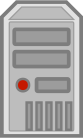
\includegraphics[width=.75cm]{icons/server}};

\node[right=of idsint] (routeur) {\includegraphics[width=1.25cm]{icons/router}};

\node[draw, cloud, cloud puffs = 10, cloud, minimum width=1.5cm,minimum height=1cm,below=of routeur] (cloud) {};

\node[right=of routeur] (idsdmz) {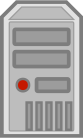
\includegraphics[width=.75cm]{icons/server}};
\node[right=of idsdmz] (dmz) {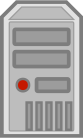
\includegraphics[width=.75cm]{icons/server}};

%% NETWORKS
\draw[thick] (client) -- node[ethernet, at start]{eth0} node[ethernet, at end]{eth1} (idsint) node[network,midway] {192.168.0.0};

\draw[thick] (idsint) -- node[ethernet, at start]{eth0} node[ethernet, at end]{eth1} (routeur) node[network,midway] {192.168.1.0};

\draw[thick] (routeur) -- node[ethernet, at start]{eth2} node[ethernet, at end]{eth0} (idsdmz) node[network,midway] {192.168.2.0};

\draw[thick] (idsdmz) -- node[ethernet, at start]{eth1} node[ethernet, at end]{eth0} (dmz) node[network,midway] {192.168.3.0};

\draw[thick] (routeur) -- node[ethernet, at start]{eth0} (cloud);

%%LABELS
\node at (0,-1) {Client};
\node at (3.1,-1) {IDS int};
\node at (9.7,-1) {IDS DMZ};
\node at (12.7,-1) {DMZ};

\node at (6.4,1) {Routeur/Pare-feu};


%% ADDRESSES
\node[address] at (.7,-.5) {.5};
\node[address] at (2.4,-.5) {.254};
\node[address] at (3.8,-.5) {.10};
\node[address] at (5.3,-.5) {.20};
\node[address] at (7.4,-.5) {.20};
\node[address] at (9,-.5) {.10};
\node[address] at (10.4,-.5) {.254};
\node[address] at (12,-.5) {.5};
\end{tikzpicture}
\end{center}

}
\subsection{Attaques \& règles de filtrage}
\frame[allowframebreaks=1.0]{
\frametitle{Attaques \& règles de filtrage}

\begin{block}{Scan avec nmap}
\begin{verbatim}
# nmap -sS 192.168.3.5
\end{verbatim}
\end{block}

\begin{exampleblock}{Règle Snort}
\begin{verbatim}
alert icmp $EXTERNAL_NET any -> $HOME_NET any ( \
msg:"DEMO-ATTACKS Scan NMAP"; dsize: 0; sid:7348;)
\end{verbatim}
\end{exampleblock}

\framebreak

\begin{block}{Injection SQL dans l'URL}
\begin{verbatim}
# links "http://192.168.3.5/index.html?login=OR 1=1"
\end{verbatim}
\end{block}

\begin{exampleblock}{Règle Snort}
\begin{verbatim}
alert tcp any any -> $HTTP_SERVERS $HTTP_PORTS ( \
msg:"DEMO-ATTACKS SQL injection"; \
uricontent:"OR 1=1"; sid:6969;)
\end{verbatim}
\end{exampleblock}

\framebreak

\begin{block}{Injection XSS dans une requête POST}
\begin{verbatim}
POST /index.html HTTP/1.0
Content-Length: 31

<script>alert("toto")</script>
\end{verbatim}
\end{block}

\begin{exampleblock}{Règle Snort}
\begin{verbatim}
alert tcp any any -> $HTTP_SERVERS $HTTP_PORTS ( \
msg:"DEMO-ATTACKS XSS attack"; content:"<script"; \
sid:7373;)
\end{verbatim}
\end{exampleblock}

\framebreak

\begin{block}{Journalisation des erreurs 403}
\begin{verbatim}
# links http://192.168.3.5/demo.html
\end{verbatim}
\end{block}

\begin{exampleblock}{Règle Snort}
\begin{verbatim}
alert tcp $HTTP_SERVERS $HTTP_PORTS -> $EXTERNAL_NET \
any (msg:"DEMO-ATTACKS 403 Forbidden"; \
content:"HTTP/1.1 403"; sid:73421;)
\end{verbatim}
\end{exampleblock}

\framebreak

\begin{block}{Fuite de /etc/passwd}
\begin{verbatim}
# links http://192.168.3.5/../etc/passwd
\end{verbatim}
\end{block}

\begin{exampleblock}{Règle Snort}
\begin{verbatim}
alert tcp any any -> $HTTP_SERVERS $HTTP_PORTS ( \
msg:"DEMO-ATTACKS /etc/passwd"; \
uricontent:"/etc/passwd"; content:"/etc/passwd"; \
sid:8455;)
\end{verbatim}
\end{exampleblock}

}

\section{Conclusion}
\frame{
\frametitle{Conclusion}


\begin{block}{Récupérer le projet}
\url{http://github.com/legrajul/projet_reseau}\\
$\hookrightarrow$ documents\\
$\hookrightarrow$ lab netkit de test
\end{block}

\begin{center}
\huge{Des questions ?}
\end{center}
}

\end{document}